\documentclass[12pt,a4paper]{article}

% ─── Page Layout ───────────────────────────────────────────────────────────────
\usepackage[a4paper, margin=0.8in, headheight=14pt]{geometry}

% ─── Fonts (XeLaTeX) ───────────────────────────────────────────────────────────
\usepackage{fontspec}
\usepackage{unicode-math}
\setmainfont{TeX Gyre Pagella}
\setmonofont[Scale=0.88]{TeX Gyre Cursor}
\setmathfont{Latin Modern Math}

% ─── Packages ──────────────────────────────────────────────────────────────────
\usepackage{xcolor}
\usepackage{colortbl}
\usepackage{titlesec}
\usepackage{enumitem}
\usepackage{tabularx}
\usepackage{booktabs}
\usepackage{array}
\usepackage{amsmath}
\usepackage{tikz}
\usetikzlibrary{shapes.geometric, arrows.meta, positioning, calc, fit, decorations.pathreplacing}
\usepackage{tcolorbox}
\tcbuselibrary{skins, breakable}
\usepackage{hyperref}
\usepackage{fancyhdr}
\usepackage{graphicx}
\usepackage{microtype}
\hyphenpenalty=10000
\exhyphenpenalty=10000
\sloppy
\usepackage{caption}
\usepackage{setspace}
\usepackage{multirow}
\usepackage{tocloft}

% ─── Q&A helper ────────────────────────────────────────────────────────────────
\newcommand{\Q}[1]{\textbf{#1}\par\noindent\ignorespaces}

% ─── Colour Palette ────────────────────────────────────────────────────────────
\definecolor{myred}{RGB}{196,30,58}
\definecolor{mydark}{RGB}{30,30,50}
\definecolor{mygreen}{RGB}{14,120,80}
\definecolor{myteal}{RGB}{0,130,140}
\definecolor{myamber}{RGB}{180,100,0}
\definecolor{mypurple}{RGB}{100,30,160}
\definecolor{mygray}{RGB}{246,247,249}
\definecolor{mgframe}{RGB}{180,185,200}
\definecolor{watermark}{RGB}{145,150,170}
\definecolor{hdrred}{RGB}{250,232,235}
\definecolor{hdrgreen}{RGB}{220,244,233}
\definecolor{hdrteal}{RGB}{220,242,244}
\definecolor{hdramber}{RGB}{253,242,215}
\definecolor{hdrpurple}{RGB}{238,228,255}
\definecolor{hdrgray}{RGB}{238,240,245}
\definecolor{rowalt}{RGB}{250,251,253}

% ─── Section Formatting ────────────────────────────────────────────────────────
\titleformat{\section}
  {\large\bfseries\color{myred}}{\thesection.}{0.5em}{}
  [\vspace{1pt}{\color{myred}\rule{\linewidth}{0.8pt}}]
\titleformat{\subsection}
  {\normalsize\bfseries\color{myteal}}{\thesubsection}{0.5em}{}
\titlespacing*{\section}{0pt}{18pt}{7pt}
\titlespacing*{\subsection}{0pt}{11pt}{4pt}

% ─── Paragraph ─────────────────────────────────────────────────────────────────
\setlength{\parindent}{0pt}
\setlength{\parskip}{4pt}

% ─── TOC Styling ───────────────────────────────────────────────────────────────
\renewcommand{\cfttoctitlefont}{\large\bfseries\color{myred}}
\renewcommand{\cftaftertoctitle}{\par\noindent{\color{myred}\rule{\linewidth}{0.8pt}}}
\setlength{\cftbeforetoctitleskip}{0pt}
\setlength{\cftaftertoctitleskip}{6pt}
\renewcommand{\cftsecfont}{\normalsize\bfseries\color{mydark}}
\renewcommand{\cftsecpagefont}{\normalsize\bfseries\color{mydark}}
\renewcommand{\cftsecleader}{\cftdotfill{\cftdotsep}}
\setlength{\cftbeforesecskip}{7pt}
\renewcommand{\cftsubsecfont}{\small\color{mydark}}
\renewcommand{\cftsubsecpagefont}{\small\color{mydark}}
\setlength{\cftbeforesubsecskip}{3pt}
\setlength{\cftsubsecindent}{1.4em}

% ─── Table helpers ─────────────────────────────────────────────────────────────
\renewcommand{\arraystretch}{1.45}
\setlength{\tabcolsep}{6pt}
\arrayrulecolor{mydark}
\newcolumntype{B}[1]{>{\small\bfseries\raggedright\arraybackslash}m{#1}}
\newcolumntype{Y}{>{\small\raggedright\arraybackslash}X}
\renewcommand{\tabularxcolumn}[1]{m{#1}}

% ─── Header / Footer ───────────────────────────────────────────────────────────
\pagestyle{fancy}
\fancyhf{}
\fancyhead[L]{\small\color{myred}\textbf{PE-EC603B}\;\color{mydark}--- Bio-Medical Electronics}
\fancyhead[R]{\small\color{myteal}\textbf{Module 3 Notes}}
\fancyfoot[C]{\small\color{mydark}\thepage}
\fancyfoot[R]{\small\color{watermark}\textit{\copyright\ Biraj}}
\renewcommand{\headrulewidth}{0.5pt}
\renewcommand{\footrulewidth}{0.3pt}

% ─── Hyperref ──────────────────────────────────────────────────────────────────
\hypersetup{
  colorlinks=true, linkcolor=myteal, urlcolor=myteal,
  pdfauthor={Biraj Sarkar},
  pdftitle={PE-EC603B --- Module 3 Notes}
}

% ─── tcolorbox styles ──────────────────────────────────────────────────────────
\tcbset{
  tikzbox/.style={
    colback=mygray, colframe=mgframe, boxrule=0.6pt, arc=4pt,
    left=8pt, right=8pt, top=6pt, bottom=6pt,
    colbacktitle=mgframe, coltitle=mydark,
    fonttitle=\small\bfseries
  },
  defbox/.style={
    colback=hdrgreen, colframe=mygreen, boxrule=0.8pt, arc=4pt,
    left=9pt, right=9pt, top=6pt, bottom=6pt,
    colbacktitle=mygreen, coltitle=white,
    fonttitle=\small\bfseries
  },
  formulabox/.style={
    colback=hdrteal, colframe=myteal, boxrule=0.8pt, arc=4pt,
    left=9pt, right=9pt, top=7pt, bottom=7pt,
    colbacktitle=myteal, coltitle=white,
    fonttitle=\small\bfseries
  },
  examplebox/.style={
    colback=hdramber, colframe=myamber, boxrule=0.8pt, arc=4pt,
    left=9pt, right=9pt, top=6pt, bottom=6pt,
    colbacktitle=myamber, coltitle=white,
    fonttitle=\small\bfseries
  },
  masonbox/.style={
    colback=hdrpurple, colframe=mypurple, boxrule=0.8pt, arc=4pt,
    left=9pt, right=9pt, top=6pt, bottom=6pt,
    colbacktitle=mypurple, coltitle=white,
    fonttitle=\small\bfseries
  },
  exambox/.style={
    colback=hdrpurple, colframe=mypurple, boxrule=1pt, arc=5pt,
    left=10pt, right=10pt, top=8pt, bottom=8pt,
    colbacktitle=mypurple, coltitle=white,
    fonttitle=\bfseries,
    breakable, title after break={\textbf{Frequently Asked / Viva Questions (contd.)}}}
}
\tcbset{breakable}

% ─── TikZ styles ───────────────────────────────────────────────────────────────
\tikzset{
  block/.style={rectangle, draw=myteal, fill=hdrteal,
    text width=2.4cm, align=center, minimum height=0.95cm,
    font=\small, rounded corners=3pt, line width=0.7pt},
  redblock/.style={rectangle, draw=myred, fill=hdrred,
    text width=2.4cm, align=center, minimum height=0.95cm,
    font=\small, rounded corners=3pt, line width=0.7pt},
  greenblock/.style={rectangle, draw=mygreen, fill=hdrgreen,
    text width=2.4cm, align=center, minimum height=0.95cm,
    font=\small, rounded corners=3pt, line width=0.7pt},
  amberblock/.style={rectangle, draw=myamber, fill=hdramber,
    text width=2.4cm, align=center, minimum height=0.95cm,
    font=\small, rounded corners=3pt, line width=0.7pt},
  purpblock/.style={rectangle, draw=mypurple, fill=hdrpurple,
    text width=2.4cm, align=center, minimum height=0.95cm,
    font=\small, rounded corners=3pt, line width=0.7pt},
  sumjunc/.style={circle, draw=myamber, fill=hdramber,
    minimum size=0.62cm, font=\small, line width=0.8pt},
  arrow/.style={-Stealth, thick, color=mydark},
  redarrow/.style={-Stealth, thick, color=myred},
  line/.style={thick, color=mydark}
}

% ═══════════════════════════════════════════════════════════════════════════════
\begin{document}
% ═══════════════════════════════════════════════════════════════════════════════

\begin{center}
  {\LARGE\bfseries\color{myred} PE-EC603B --- Bio-Medical Electronics}\\[5pt]
  {\normalsize\color{mydark} Semester VI \quad$\bullet$\quad 3L:0T:0P \quad$\bullet$\quad 3 Credits}\\[3pt]
  {\normalsize\color{myteal}\textbf{Module 3 Exam Notes: Physiological Measurement and Medical Imaging}}\\[3pt]
  {\small\color{mydark} CGEC \;$|$\; B.Tech ECE (2023--27) \;$|$\; \textit{Biraj Sarkar}}
\end{center}
\vspace{2pt}
\noindent{\color{myred}\rule{\linewidth}{1.5pt}}
\vspace{2pt}

\hypersetup{linkcolor=mydark}
\tableofcontents
\hypersetup{linkcolor=myteal}
\newpage

% ===============================================================================
\section{Blood Temperature Measurement}
% ===============================================================================

\begin{tcolorbox}[defbox, title={\textbf{Body Temperature and Its Clinical Significance}}]
Normal core body temperature is $37\,^{\circ}\text{C}$ (oral: $36.8\,^{\circ}\text{C}$; rectal: $37.5\,^{\circ}\text{C}$). Pyrexia (fever $> 37.5\,^{\circ}\text{C}$) and hypothermia ($< 35\,^{\circ}\text{C}$) are important clinical indicators. Core temperature is measured at the tympanic membrane, oesophagus, nasopharynx, pulmonary artery (Swan-Ganz catheter), or rectum.
\end{tcolorbox}

\subsection{Methods of Blood / Core Temperature Measurement}

\par\noindent
\begin{tabularx}{\linewidth}{|B{3.0cm}|Y|Y|}
\hline
\textbf{Method} & \textbf{\color{myteal}Principle / Sensor} & \textbf{\color{mygreen}Site / Accuracy} \\
\hline
\textbf{Thermistor probe} & NTC semiconductor; resistance drops as temperature rises. & Rectal, oesophageal, urinary bladder. Accuracy: $\pm 0.1\,^{\circ}$C. \\
\hline
\textbf{Thermocouple} & Seebeck effect; voltage proportional to temperature difference between junction and reference. & Pulmonary artery catheter, cardiac surgery. \\
\hline
\textbf{Tympanic IR} & Infrared radiation from tympanic membrane detected by thermopile; proportional to temperature. & Ear canal. Fast ($<2\,\text{s}$), non-invasive. \\
\hline
\textbf{Liquid crystal} & Liquid crystal phase transition indicates temperature by colour change. & Forehead strips. Low accuracy ($\pm 0.5\,^{\circ}$C). \\
\hline
\end{tabularx}

\textbf{Thermodilution (for cardiac output):} Cold saline is injected into the right atrium; a thermistor at the pulmonary artery tip detects the temperature drop as a function of time. Cardiac output is calculated using the \textbf{Stewart-Hamilton equation}:
\[
CO = \frac{V_{inj}(T_B - T_{inj}) \cdot K}{\int_0^\infty \Delta T_B(t)\,dt}
\]
where $V_{inj}$ = injected volume, $T_B$ = blood temperature, $T_{inj}$ = injectate temperature, $K$ = correction constant.

% ===============================================================================
\section{Blood Pressure Measurement}
% ===============================================================================

\begin{tcolorbox}[defbox, title={\textbf{Blood Pressure}}]
\textbf{Blood pressure (BP)} is the force exerted by circulating blood against the walls of blood vessels. Normal arterial BP is expressed as systolic/diastolic: $120/80\,\text{mmHg}$. It is measured directly (invasively) by intravascular catheter or indirectly (non-invasively) by sphygmomanometer.
\end{tcolorbox}

\subsection{Invasive (Direct) Blood Pressure Measurement}

A fluid-filled catheter is inserted into an artery and connected to an external strain-gauge pressure transducer (or has a miniature tip-mounted sensor). The transducer converts the pressure waveform into a voltage signal displayed continuously.

\textbf{Advantages:} Continuous beat-to-beat waveform, accurate even in shock states. \\
\textbf{Disadvantage:} Infection risk, arterial injury, thrombosis.

\subsection{Non-Invasive (Indirect) Blood Pressure Measurement}

\textbf{Sphygmomanometer with Korotkoff Sounds Method:}
\begin{enumerate}[leftmargin=*, itemsep=3pt]
  \item An inflatable cuff is placed around the upper arm and inflated above systolic pressure $\to$ artery collapses, no blood flow, no sound.
  \item Cuff pressure slowly deflated. When cuff pressure falls to systolic pressure, blood spurts through partially occluded artery $\to$ \textbf{first Korotkoff sound} heard (tapping). This pressure = \textbf{Systolic BP}.
  \item As cuff pressure continues to fall, sounds change (tapping $\to$ swishing $\to$ dull thumping).
  \item When cuff pressure drops to diastolic pressure, the artery is fully open $\to$ \textbf{sounds disappear}. This pressure = \textbf{Diastolic BP}.
\end{enumerate}

\begin{tcolorbox}[tikzbox, title={Blood Pressure Waveform --- Systolic, Diastolic and Pulse Pressure}]
\centering
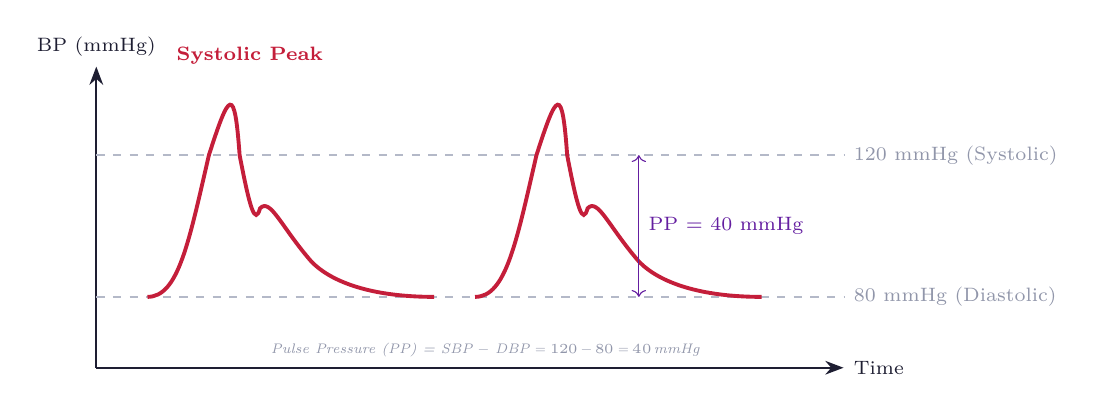
\begin{tikzpicture}[x=1.3cm, y=0.045cm, thick]
  \draw[arrow] (-0.3, 60) -- (-0.3, 145) node[above, font=\scriptsize] {BP (mmHg)};
  \draw[arrow] (-0.3, 60) -- (7.0, 60) node[right, font=\scriptsize] {Time};

  % Reference lines
  \draw[dashed, color=mgframe] (-0.3, 120) -- (7.0, 120) node[right, font=\scriptsize, color=watermark] {120 mmHg (Systolic)};
  \draw[dashed, color=mgframe] (-0.3, 80) -- (7.0, 80) node[right, font=\scriptsize, color=watermark] {80 mmHg (Diastolic)};

  % One cardiac cycle waveform, repeated twice
  \foreach \xoff in {0, 3.2} {
    \draw[color=myred, line width=1.4pt]
      (\xoff+0.2, 80)
      .. controls (\xoff+0.5, 80) and (\xoff+0.6, 95) .. (\xoff+0.8, 120)
      .. controls (\xoff+1.0, 138) and (\xoff+1.05, 140) .. (\xoff+1.1, 120)
      .. controls (\xoff+1.2, 105) and (\xoff+1.25, 100) .. (\xoff+1.3, 105)
      .. controls (\xoff+1.4, 108) and (\xoff+1.5, 100) .. (\xoff+1.8, 90)
      .. controls (\xoff+2.0, 84) and (\xoff+2.4, 80) .. (\xoff+3.0, 80);
  }

  % Labels
  \node[font=\scriptsize\bfseries, color=myred] at (1.2, 148) {Systolic Peak};
  \draw[<->, color=mypurple, thin] (5.0, 80) -- (5.0, 120) node[midway, right, font=\scriptsize, color=mypurple] {PP = 40 mmHg};

  % Annotation
  \node[font=\tiny\itshape, color=watermark] at (3.5, 65) {Pulse Pressure (PP) = SBP $-$ DBP $= 120-80 = 40\,\text{mmHg}$};
\end{tikzpicture}
\end{tcolorbox}

\textbf{Oscillometric Method (Automated NIBP monitors):} The cuff is inflated and deflated automatically. A pressure sensor in the monitor detects the oscillations of the arterial wall transmitted through the cuff. Maximum oscillation occurs at \textbf{MAP} (Mean Arterial Pressure). Systolic and diastolic pressures are computed algorithmically.

\begin{tcolorbox}[formulabox, title={\textbf{Blood Pressure Formulas}}]
\renewcommand{\arraystretch}{1.3}
\begin{tabularx}{\linewidth}{B{3.8cm} X}
Pulse Pressure & $PP = SBP - DBP = 120 - 80 = 40\,\text{mmHg}$ \\[4pt]
Mean Arterial Pressure & $MAP = DBP + \dfrac{PP}{3} = 80 + \dfrac{40}{3} \approx 93\,\text{mmHg}$ \\[8pt]
Alternatively & $MAP = \dfrac{SBP + 2 \times DBP}{3}$
\end{tabularx}
\end{tcolorbox}

% ===============================================================================
\section{Blood Flow Measurement}
% ===============================================================================

\subsection{Electromagnetic Flowmeter (Review)}

Based on Faraday's law: $V_{emf} = Bvd$ (covered in Module 2). Used intraoperatively to measure coronary or renal artery blood flow.

\subsection{Plethysmography}

\begin{tcolorbox}[defbox, title={\textbf{Plethysmography}}]
\textbf{Plethysmography} is the measurement of changes in \textbf{volume} of a body part or organ, used to assess blood flow and venous function. It detects volumetric pulsations caused by arterial inflow exceeding venous outflow during systole.
\end{tcolorbox}

\textbf{Types:} (a) \textbf{Strain-gauge plethysmography:} A mercury-in-silastic gauge around the limb stretches with each pulse, changing resistance $\propto$ volume change. (b) \textbf{Photo-plethysmography (PPG):} Light from an LED is transmitted through or reflected from the tissue; the varying absorption of the pulsatile blood volume modulates the photodetector output. Basis of pulse oximetry.

% ===============================================================================
\section{Impedance Plethysmography}
% ===============================================================================

\begin{tcolorbox}[defbox, title={\textbf{Impedance Plethysmography}}]
\textbf{Impedance plethysmography} measures changes in the \textbf{electrical impedance} of a body segment (typically the thorax or a limb) to infer changes in blood volume or respiratory activity. Blood has a lower resistivity than surrounding tissue, so arterial blood inflow during systole decreases the measured impedance.
\end{tcolorbox}

\subsection{Principle}

A high-frequency ($20$--$100\,\text{kHz}$), low-amplitude ($1$--$4\,\text{mA}$ rms) alternating current is injected through outer electrodes. The voltage is sensed by inner (pick-up) electrodes, and the impedance $Z = V/I$ is computed. Changes in blood volume produce small, rhythmic changes in impedance $\Delta Z$.

\subsection{Nyboer's Formula (Limb Blood Flow)}

\begin{tcolorbox}[formulabox, title={\textbf{Impedance Plethysmography Formulas}}]
\[
\Delta V = \frac{\rho_b \cdot L^2}{Z_0^2} \cdot \Delta Z
\]
where: $\Delta V$ = change in blood volume (mL), $\rho_b$ = resistivity of blood ($\approx 150\,\Omega\cdot\text{cm}$), $L$ = segment length (cm), $Z_0$ = baseline impedance ($\Omega$), $\Delta Z$ = impedance change ($\Omega$). \\[6pt]
\textbf{Impedance Cardiography (ICG)} measures stroke volume and cardiac output non-invasively from thoracic impedance changes.
\end{tcolorbox}

\begin{tcolorbox}[tikzbox, title={Impedance Plethysmography --- 4-Electrode Configuration}]
\centering
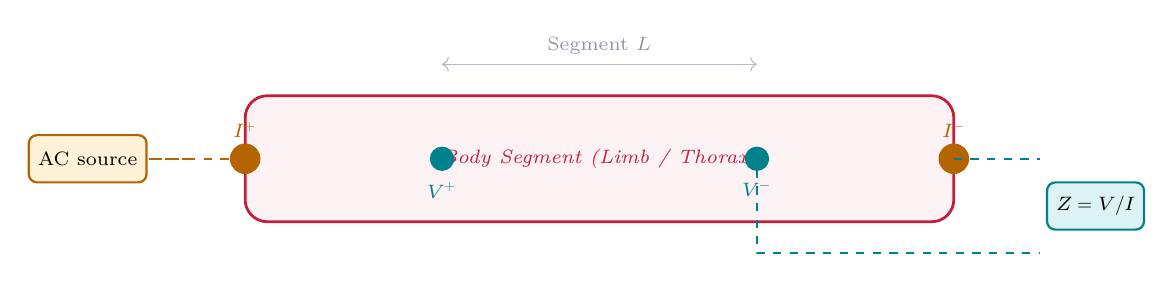
\begin{tikzpicture}[thick, font=\small]
  % Limb segment (rectangle)
  \filldraw[fill=hdrred!60, draw=myred, rounded corners=8pt, line width=1pt]
    (-4.5, -0.8) rectangle (4.5, 0.8);
  \node[font=\scriptsize\itshape, color=myred] at (0, 0) {Body Segment (Limb / Thorax)};

  % Outer current injection electrodes (I+ and I-)
  \filldraw[fill=myamber, draw=myamber] (-4.5, 0) circle (0.18) node[above=4pt, font=\scriptsize\bfseries, color=myamber] {$I^+$};
  \filldraw[fill=myamber, draw=myamber] (4.5, 0) circle (0.18) node[above=4pt, font=\scriptsize\bfseries, color=myamber] {$I^-$};

  % Inner voltage sense electrodes (V+ and V-)
  \filldraw[fill=myteal, draw=myteal] (-2.0, 0) circle (0.14) node[below=5pt, font=\scriptsize\bfseries, color=myteal] {$V^+$};
  \filldraw[fill=myteal, draw=myteal] (2.0, 0) circle (0.14) node[below=5pt, font=\scriptsize\bfseries, color=myteal] {$V^-$};

  % Current source (left)
  \draw[color=myamber, dashed] (-4.5, 0) -- (-5.8, 0);
  \node[draw=myamber, fill=hdramber, rounded corners=3pt, font=\scriptsize, minimum width=1.0cm, minimum height=0.6cm]
    at (-6.5, 0) {AC source};
  \draw[color=myamber, dashed] (-5.2, 0) -- (-5.8, 0);

  % Voltage sense amplifier (right)
  \draw[color=myteal, dashed] (4.5, 0) -- (5.6, 0);
  \draw[color=myteal, dashed] (2.0, -0.14) -- (2.0, -1.2) -- (5.6, -1.2);
  \node[draw=myteal, fill=hdrteal, rounded corners=3pt, font=\scriptsize, minimum width=1.2cm, minimum height=0.6cm]
    at (6.3, -0.6) {$Z = V/I$};

  % Spacing label
  \draw[<->, color=mgframe, thin] (-2.0, 1.2) -- (2.0, 1.2) node[midway, above, font=\scriptsize, color=watermark] {Segment $L$};
\end{tikzpicture}
\end{tcolorbox}

\textbf{Clinical Applications of Impedance Plethysmography:}
\begin{itemize}[leftmargin=*, itemsep=2pt]
  \item \textbf{Cardiac output} measurement (non-invasive impedance cardiography).
  \item \textbf{Respiratory rate and tidal volume} monitoring (thoracic impedance changes with breathing).
  \item \textbf{Deep Vein Thrombosis (DVT)} detection by venous occlusion impedance plethysmography.
  \item \textbf{Body composition analysis} (bioelectrical impedance analysis, BIA).
\end{itemize}

% ===============================================================================
\section{Ultrasonic Imaging}
% ===============================================================================

\begin{tcolorbox}[defbox, title={\textbf{Ultrasonic Imaging}}]
\textbf{Ultrasonic imaging} uses high-frequency sound waves ($1$--$20\,\text{MHz}$) generated by piezoelectric transducers to visualize internal body structures. Sound waves are reflected at tissue interfaces (impedance mismatch), and the time of return (echo) and amplitude are used to construct images.
\end{tcolorbox}

\subsection{Acoustic Impedance and Reflection}

\begin{tcolorbox}[formulabox, title={\textbf{Ultrasound Key Formulas}}]
\renewcommand{\arraystretch}{1.3}
\begin{tabularx}{\linewidth}{B{3.8cm} X}
Speed of sound in tissue & $c \approx 1540\,\text{m/s}$ (average soft tissue). \\[4pt]
Acoustic impedance & $Z = \rho \cdot c$ \quad ($\rho$ = density, kg/m$^3$) \\[4pt]
Reflection coefficient & $R = \left(\dfrac{Z_2 - Z_1}{Z_2 + Z_1}\right)^2$ \\[8pt]
Depth of reflector & $d = \dfrac{c \cdot t}{2}$ \quad ($t$ = round-trip travel time) \\[4pt]
Axial resolution & $\Delta z = \dfrac{c}{2B}$ \quad ($B$ = pulse bandwidth) \\[4pt]
Doppler shift & $\Delta f = \dfrac{2 f_0 v \cos\theta}{c}$
\end{tabularx}
\end{tcolorbox}

\subsection{Modes of Ultrasonic Imaging}

\par\noindent
\begin{tabularx}{\linewidth}{|B{2.0cm}|Y|Y|}
\hline
\textbf{Mode} & \textbf{\color{myteal}Description} & \textbf{\color{mygreen}Application} \\
\hline
A-mode (Amplitude) & Echoes displayed as amplitude spikes vs.\ time. 1D range measurement. & Ophthalmology (eye axial length); echoencephalography. \\
\hline
B-mode (Brightness) & Echo amplitude coded as brightness; 2D scan built by sweeping the beam. & Standard abdominal, obstetric ultrasound; liver, kidney, uterus. \\
\hline
M-mode (Motion) & Single beam; echoes displayed as position vs.\ time graph. Captures motion. & Echocardiography: cardiac valve motion, chamber dimension. \\
\hline
Doppler (Colour Flow) & Blood velocity colour-coded (red = towards, blue = away) overlaid on B-mode. & Vascular studies, cardiac valve regurgitation, stenosis. \\
\hline
3D / 4D & Multiple 2D planes reconstructed into 3D volume; 4D adds real-time motion. & Fetal morphology, cardiac volume assessment. \\
\hline
\end{tabularx}

\begin{tcolorbox}[tikzbox, title={Ultrasound Imaging System Block Diagram}]
\centering
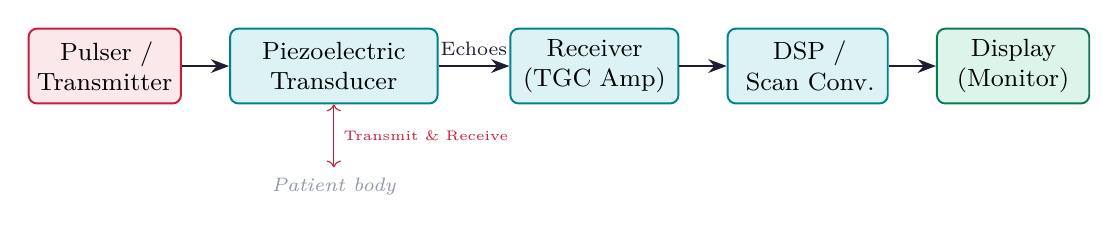
\begin{tikzpicture}[thick, font=\small,
  sblock/.style={rectangle, draw=myteal, fill=hdrteal,
    align=center, minimum height=0.95cm, font=\small,
    rounded corners=3pt, line width=0.7pt},
  spulser/.style={rectangle, draw=myred, fill=hdrred,
    align=center, minimum height=0.95cm, font=\small,
    rounded corners=3pt, line width=0.7pt},
  sdisp/.style={rectangle, draw=mygreen, fill=hdrgreen,
    align=center, minimum height=0.95cm, font=\small,
    rounded corners=3pt, line width=0.7pt}]

  \node[spulser, text width=1.7cm] (pulser) {Pulser /\\Transmitter};
  \node[sblock, right=0.6cm of pulser, text width=2.4cm] (xdcr) {Piezoelectric\\Transducer};
  \node[sblock, right=0.9cm of xdcr, text width=1.9cm] (recv) {Receiver\\(TGC Amp)};
  \node[sblock, right=0.6cm of recv, text width=1.8cm] (dsp) {DSP /\\Scan Conv.};
  \node[sdisp, right=0.6cm of dsp, text width=1.7cm] (disp) {Display\\(Monitor)};

  % Arrows
  \draw[arrow] (pulser) -- (xdcr);
  \draw[arrow] (xdcr) -- node[above, font=\scriptsize] {Echoes} (recv);
  \draw[arrow] (recv) -- (dsp);
  \draw[arrow] (dsp) -- (disp);

  % Body annotation
  \node[font=\scriptsize\itshape, color=watermark, below=0.8cm of xdcr] (body) {Patient body};
  \draw[<->, color=myred, thin] (xdcr.south) -- (body.north) node[midway, right, font=\tiny, color=myred] {Transmit \& Receive};
\end{tikzpicture}
\end{tcolorbox}

\textbf{Time-Gain Compensation (TGC):} Echoes from deeper structures are weaker due to attenuation. TGC amplifies echoes by an increasing gain as a function of time (depth) to equalize the displayed brightness across depth. Typical attenuation: $\approx 0.5\,\text{dB/cm/MHz}$.

% ===============================================================================
\section{X-ray Imaging}
% ===============================================================================

\begin{tcolorbox}[defbox, title={\textbf{X-ray Imaging}}]
\textbf{X-rays} are electromagnetic radiation ($0.01$--$10\,\text{nm}$ wavelength; $10^{16}$--$10^{19}\,\text{Hz}$) generated by bombarding a tungsten anode with high-velocity electrons. They penetrate tissue differentially based on tissue density and atomic number, creating a projected shadow image.
\end{tcolorbox}

\subsection{Attenuation Law}

\begin{tcolorbox}[formulabox, title={\textbf{Beer-Lambert Law for X-rays}}]
\[
I = I_0 \cdot e^{-\mu x}
\]
where $I_0$ = incident X-ray intensity, $I$ = transmitted intensity, $\mu$ = linear attenuation coefficient (cm$^{-1}$, depends on material and photon energy), $x$ = thickness of material (cm).
\end{tcolorbox}

\textbf{Tissue Contrast:} Bone ($\mu$ high, appears white) $>$ Soft tissue $>$ Fat $>$ Air ($\mu$ low, appears black).

\subsection{Computed Tomography (CT)}

\begin{tcolorbox}[defbox, title={\textbf{Computed Tomography (CT)}}]
\textbf{CT} (Computerised Tomography, or CAT scan) uses a rotating X-ray source and a detector array to acquire many projections at different angles. A reconstruction algorithm (\textbf{filtered back-projection} or iterative methods) produces cross-sectional (axial) images of the body. CT values are expressed in \textbf{Hounsfield Units (HU)}: water $= 0\,\text{HU}$, air $= -1000\,\text{HU}$, bone $= +400$ to $+1000\,\text{HU}$.
\end{tcolorbox}

\textbf{Advantages of CT over plain X-ray:} Cross-sectional images eliminate overlapping structures; better soft tissue contrast with contrast agents; enables 3D reconstruction.

\textbf{Radiation dose:} CT delivers a significantly higher dose than plain X-ray (chest CT $\approx 7\,\text{mSv}$ vs.\ chest X-ray $\approx 0.1\,\text{mSv}$).

% ===============================================================================
\section{Nuclear Imaging}
% ===============================================================================

\begin{tcolorbox}[defbox, title={\textbf{Nuclear (Radionuclide) Imaging}}]
\textbf{Nuclear imaging} introduces a radioactive tracer (\textbf{radiopharmaceutical}) into the patient. The tracer accumulates in target tissues (e.g., tumour, heart). Gamma rays emitted by the tracer are detected externally to create functional images showing organ physiology and metabolism rather than anatomy alone.
\end{tcolorbox}

\subsection{Scintigraphy and Gamma Camera}

A radiotracer (e.g., Technetium-99m, $^{99m}$Tc, emitting $140\,\text{keV}$ gamma rays) is injected. The \textbf{gamma camera (Anger camera)} uses a large NaI(Tl) scintillator crystal coupled to an array of photomultiplier tubes (PMTs) to detect and locate each gamma photon. A collimator ensures only perpendicularly incident photons reach the crystal. The image represents tracer distribution in the organ.

\subsection{SPECT (Single Photon Emission Computed Tomography)}

A gamma camera rotates around the patient, acquiring multiple projections. 3D images are reconstructed similarly to CT. Used for: myocardial perfusion imaging (heart), brain SPECT (epilepsy, dementia), bone scans.

\subsection{PET (Positron Emission Tomography)}

\begin{tcolorbox}[defbox, title={\textbf{PET Scanning}}]
\textbf{PET} uses positron-emitting radiotracers (e.g., $^{18}$F-FDG, a glucose analogue). The emitted positron annihilates with an electron, producing two $511\,\text{keV}$ gamma photons travelling in \textbf{opposite directions} ($180^{\circ}$). Coincidence detection of both photons defines the line of response without a collimator, giving higher sensitivity and resolution than SPECT.
\end{tcolorbox}

\par\noindent
\begin{tabularx}{\linewidth}{|B{2.2cm}|Y|Y|Y|}
\hline
\textbf{Technique} & \textbf{\color{myteal}Radiation} & \textbf{\color{myamber}Resolution} & \textbf{\color{mygreen}Key Application} \\
\hline
\textbf{X-ray} & X-ray photons & 0.1 mm & Bone fractures, chest pathology. \\
\hline
\textbf{CT} & X-ray photons & 0.5--1 mm & Trauma, lung, abdominal, 3D anatomy. \\
\hline
\textbf{Scintigraphy} & $\gamma$ rays (single) & 10--15 mm & Bone scans, thyroid function. \\
\hline
\textbf{SPECT} & $\gamma$ rays (single) & 7--10 mm & Cardiac perfusion, brain function. \\
\hline
\textbf{PET} & $\gamma$ rays (coincidence) & 3--5 mm & Oncology (tumour), brain metabolism. \\
\hline
\textbf{PET-CT} & Combined & 3--5 mm & Anatomy + Function fusion; gold standard in oncology. \\
\hline
\end{tabularx}

\newpage
% ===============================================================================
% MANDATORY QUICK REVISION PAGE
% ===============================================================================
\begin{center}
  {\large\bfseries\color{myred} Quick Revision --- Module 3}\\[3pt]
  {\small\color{mydark} Physiological Measurement and Medical Imaging $|$ PE-EC603B}
\end{center}
\noindent{\color{myred}\rule{\linewidth}{1.2pt}}
\vspace{4pt}

\begin{tcolorbox}[formulabox, title={\textbf{Key Formulas}}]
\renewcommand{\arraystretch}{1.3}
\begin{tabularx}{\linewidth}{B{4.0cm} X}
Mean Arterial Pressure & $MAP = DBP + PP/3 = (SBP + 2\,DBP)/3$ \\[4pt]
Pulse Pressure & $PP = SBP - DBP$ \\[4pt]
Thermodilution CO & $CO = \dfrac{V_{inj}(T_B - T_{inj})\cdot K}{\int \Delta T_B\,dt}$ \\[8pt]
Impedance plethysm. & $\Delta V = \dfrac{\rho_b L^2}{Z_0^2}\Delta Z$ \\[8pt]
Ultrasound depth & $d = ct/2$ \\[4pt]
Acoustic impedance & $Z = \rho c$ \\[4pt]
Reflection coeff. & $R = \left(\dfrac{Z_2-Z_1}{Z_2+Z_1}\right)^2$ \\[8pt]
X-ray attenuation & $I = I_0 e^{-\mu x}$ \\[4pt]
Doppler shift & $\Delta f = 2f_0 v\cos\theta / c$
\end{tabularx}
\end{tcolorbox}

\begin{tcolorbox}[defbox, title={\textbf{One-Line Definitions}}]
\begin{itemize}[leftmargin=*, itemsep=2.5pt, topsep=0pt]
  \item \textbf{Korotkoff Sounds:} Sounds heard through a stethoscope during sphygmomanometer BP measurement; first sound = systolic BP; disappearance = diastolic BP.
  \item \textbf{Pulse Pressure:} Difference between systolic and diastolic BP ($\approx 40\,\text{mmHg}$).
  \item \textbf{Impedance Plethysmography:} Measures blood volume changes via electrical impedance changes of a body segment.
  \item \textbf{TGC (Time-Gain Compensation):} Increasing amplifier gain with time to compensate for ultrasound attenuation at greater depths.
  \item \textbf{Acoustic Impedance:} Product of tissue density and sound velocity ($Z = \rho c$); mismatch between tissues causes ultrasound reflection.
  \item \textbf{Hounsfield Unit:} Standardized scale of X-ray attenuation in CT; water = 0 HU, air = $-1000$ HU.
  \item \textbf{Scintigraphy:} 2D nuclear imaging using a gamma camera after radiopharmaceutical injection.
  \item \textbf{PET:} Positron Emission Tomography; uses annihilation coincidence detection of two $511\,\text{keV}$ photons for 3D functional imaging.
  \item \textbf{A-mode ultrasound:} One-dimensional distance measurement from echo amplitude spikes on a time axis.
  \item \textbf{B-mode ultrasound:} 2D grey-scale image formed by brightness-coding echo amplitude as the beam is swept.
\end{itemize}
\end{tcolorbox}

\begin{tcolorbox}[exambox, title={\textbf{Frequently Asked / Viva Questions}}]
\begin{enumerate}[topsep=0pt, label=\textbf{Q\arabic*.}, itemsep=5pt]
  \item \Q{Describe the Korotkoff sound method for non-invasive blood pressure measurement.}
    A cuff is inflated above systolic pressure (artery occluded; no sound). As cuff deflates, the first tapping Korotkoff sound marks \textit{systolic BP}. Sounds change character until they disappear entirely at \textit{diastolic BP}, when the artery is fully open.
  \item \Q{What is the oscillometric method of blood pressure measurement?}
    An automated cuff inflates and deflates. A pressure sensor detects oscillations from the arterial wall transmitted through cuff air. Maximum oscillation amplitude occurs at MAP. Systolic and diastolic pressures are computed by algorithm from the oscillation envelope.
  \item \Q{Define Mean Arterial Pressure and give its formula.}
    MAP is the average arterial pressure over one cardiac cycle, weighted for the longer diastolic phase: $MAP = DBP + PP/3 \approx 93\,\text{mmHg}$. Alternatively $MAP = (SBP + 2\times DBP)/3$.
  \item \Q{What is impedance plethysmography? State the Nyboer formula.}
    It measures blood volume changes by injecting a safe high-frequency AC current and detecting impedance changes: $\Delta V = \rho_b L^2 \Delta Z / Z_0^2$. Arterial inflow during systole decreases impedance; respiratory motion also changes thoracic impedance.
  \item \Q{Explain acoustic impedance and its role in ultrasound imaging.}
    Acoustic impedance $Z = \rho c$. At the boundary between tissues with different $Z$, a fraction of the ultrasound energy is reflected: $R = [(Z_2-Z_1)/(Z_2+Z_1)]^2$. These reflections (echoes) form the image. At air--tissue interfaces, nearly all energy is reflected ($R \approx 1$), which is why coupling gel is essential.
  \item \Q{Compare A-mode, B-mode, and M-mode ultrasound.}
    A-mode: amplitude spikes vs.\ time for 1D depth measurement (e.g., eye). B-mode: 2D brightness map used in standard diagnostic ultrasound (abdomen, obstetrics). M-mode: single beam traces target motion over time (e.g., cardiac valve motion).
  \item \Q{State the Beer-Lambert law for X-rays and explain Hounsfield Units.}
    $I = I_0 e^{-\mu x}$. In CT, the Hounsfield Unit (HU) normalizes attenuation: water $= 0\,\text{HU}$, air $= -1000\,\text{HU}$, bone $= +400$ to $+1000\,\text{HU}$. It enables standardized comparison between scanners.
  \item \Q{What is the principle of PET scanning? How does it differ from SPECT?}
    PET uses positron-emitting tracers (e.g., $^{18}$F-FDG). Each positron annihilates with an electron to emit two $511\,\text{keV}$ photons at $180^{\circ}$. Coincidence detection defines the line of response without a collimator, giving higher sensitivity and resolution ($3$--$5\,\text{mm}$). SPECT uses a single-photon emitter and a mechanical collimator, giving lower resolution ($7$--$10\,\text{mm}$) but lower cost.
  \item \Q{Why is TGC (Time-Gain Compensation) needed in ultrasound?}
    Ultrasound is attenuated as it travels through tissue ($\approx 0.5\,\text{dB/cm/MHz}$). Deeper echoes return later and are weaker. TGC progressively increases amplifier gain with time (depth) to compensate, so that interfaces at all depths appear equally bright on the display.
  \item \Q{What is thermodilution and what does it measure?}
    Thermodilution measures cardiac output. Cold saline is injected into the right atrium; a thermistor in the pulmonary artery detects the temperature--time curve. By the Stewart-Hamilton equation, cardiac output is inversely proportional to the area under the temperature-change curve: $CO \propto 1/\int \Delta T_B\,dt$.
\end{enumerate}
\end{tcolorbox}

\begin{tcolorbox}[tikzbox, title={Imaging Modality Comparison}]
\renewcommand{\arraystretch}{1.4}
\par\noindent
\begin{tabularx}{\linewidth}{|B{2.0cm}|>{\small\centering\arraybackslash}X|>{\small\centering\arraybackslash}X|>{\small\centering\arraybackslash}X|>{\small\centering\arraybackslash}X|Y|}
\hline
\textbf{Modality} & \textbf{\color{myred}Ionizing?} & \textbf{\color{myteal}Resolution} & \textbf{\color{myamber}Image type} & \textbf{\color{mypurple}Real-time?} & \textbf{Best for} \\
\hline
X-ray & Yes & 0.1 mm & 2D shadow & No & Bone, chest \\
\hline
CT & Yes & 0.5 mm & 3D slices & No & Trauma, anatomy \\
\hline
Ultrasound & No & 0.5--2 mm & 2D/3D & Yes & Soft tissue, fetus \\
\hline
SPECT & Yes & 7--10 mm & 3D functional & No & Cardiac perfusion \\
\hline
PET & Yes & 3--5 mm & 3D metabolic & No & Oncology, brain \\
\hline
MRI & No & 0.5--1 mm & 3D anatomy & No & Brain, soft tissue \\
\hline
\end{tabularx}
\end{tcolorbox}

\end{document}
